\documentclass[10pt,a4paper]{article}

\usepackage[T1]{fontenc}
\usepackage[utf8]{inputenc}
\usepackage[english]{babel}
\usepackage[sc]{mathpazo}
\usepackage{microtype}
\usepackage[a4paper,margin=2.1cm,top=1.9cm,bottom=1.9cm]{geometry}
\usepackage{amsmath,amssymb}
\usepackage{graphicx}
\usepackage{booktabs,tabularx,makecell}
\usepackage{enumitem}
\usepackage[font=small,labelfont=bf,labelsep=colon,skip=3pt]{caption}
\usepackage{xcolor}
\usepackage[most]{tcolorbox}
\usepackage[hidelinks]{hyperref}
\usepackage{float}
\usepackage{url}

\definecolor{blueI}{HTML}{2A78D6}
\newtcolorbox{summary}{enhanced, breakable, colback=blueI!5!white, colframe=blueI, boxrule=0pt,
  leftrule=2.4pt, arc=0pt, outer arc=0pt, left=6pt, right=6pt, top=3pt, bottom=3pt}
\newtcolorbox{reading}{enhanced, breakable, colback=black!3!white, colframe=black!45, boxrule=0pt,
  leftrule=1.6pt, arc=0pt, outer arc=0pt, left=5pt, right=5pt, top=2pt, bottom=2pt, fontupper=\small}

\graphicspath{{../out/d120_eh500_ez300_th45_g120_q0.1/}{../../../ideas/group-identification/figures/}}
\newcommand{\G}{\mathrm{G}}
\newcommand{\A}{\mathrm{A}}
\newcommand{\Sl}{\mathrm{S}}
\setlist{itemsep=1pt, topsep=2pt, parsep=0pt, leftmargin=1.3em}
\setlength{\parindent}{0pt}
\setlength{\parskip}{3pt}
\captionsetup{font=footnotesize}
\newcommand{\Abreast}{35}
\newcommand{\AtDeparture}{1\,179}
\newcommand{\AtLanding}{1\,358}
\newcommand{\ClimbA}{29.1}
\newcommand{\ClimbG}{33.0}
\newcommand{\ClimbS}{30.8}
\newcommand{\DClimbFlight}{$+$5.71}
\newcommand{\DClimbFlightBand}{[$+$5.52, $+$5.92]}
\newcommand{\DClimbGroupSdh}{$+$3.28}
\newcommand{\DClimbGroupSdhBand}{[$+$3.11, $+$3.47]}
\newcommand{\DClimbRaw}{$+$2.20}
\newcommand{\DClimbRawBand}{[$+$1.96, $+$2.45]}
\newcommand{\DClimbSdh}{$+$3.43}
\newcommand{\DClimbSdhBand}{[$+$3.19, $+$3.63]}
\newcommand{\DClimbSel}{$+$0.43}
\newcommand{\DClimbSelBand}{[$+$0.25, $+$0.59]}
\newcommand{\DClimbSizeMax}{$+$4.0}
\newcommand{\DClimbSizeMin}{$+$2.0}
\newcommand{\DCompClimb}{$-$1.23}
\newcommand{\DCompFound}{$+$2.06}
\newcommand{\DCompHlocHundred}{$+$0.006}
\newcommand{\DCompHlocThousand}{$+$0.014}
\newcommand{\DCompRate}{$+$0.009}
\newcommand{\DCompSink}{$-$8.6}
\newcommand{\DCompSpeed}{$+$1.20}
\newcommand{\DCompXc}{$+$0.55}
\newcommand{\DFoundFlight}{$+$8.75}
\newcommand{\DFoundFlightBand}{[$+$8.37, $+$9.15]}
\newcommand{\DFoundGroupSdh}{$+$2.59}
\newcommand{\DFoundGroupSdhBand}{[$+$2.25, $+$2.99]}
\newcommand{\DFoundRaw}{$+$6.18}
\newcommand{\DFoundRawBand}{[$+$5.82, $+$6.46]}
\newcommand{\DFoundSdh}{$+$4.12}
\newcommand{\DFoundSdhBand}{[$+$3.68, $+$4.54]}
\newcommand{\DFoundSel}{$+$1.60}
\newcommand{\DFoundSelBand}{[$+$1.23, $+$1.97]}
\newcommand{\DHlocHundredFlight}{$-$0.009}
\newcommand{\DHlocHundredFlightBand}{[$-$0.009, $-$0.008]}
\newcommand{\DHlocHundredGroupSdh}{$+$0.002}
\newcommand{\DHlocHundredGroupSdhBand}{[$+$0.001, $+$0.002]}
\newcommand{\DHlocHundredRaw}{$+$0.008}
\newcommand{\DHlocHundredRawBand}{[$+$0.007, $+$0.009]}
\newcommand{\DHlocHundredSdh}{$+$0.002}
\newcommand{\DHlocHundredSdhBand}{[$+$0.001, $+$0.003]}
\newcommand{\DHlocHundredSel}{$+$0.005}
\newcommand{\DHlocHundredSelBand}{[$+$0.004, $+$0.005]}
\newcommand{\DHlocThousandFlight}{$+$0.037}
\newcommand{\DHlocThousandFlightBand}{[$+$0.035, $+$0.039]}
\newcommand{\DHlocThousandFlightSeven}{$+$0.087}
\newcommand{\DHlocThousandFlightSevenBand}{[$+$0.069, $+$0.105]}
\newcommand{\DHlocThousandFlightTwo}{$+$0.026}
\newcommand{\DHlocThousandFlightTwoBand}{[$+$0.023, $+$0.029]}
\newcommand{\DHlocThousandGroupSdh}{$+$0.043}
\newcommand{\DHlocThousandGroupSdhBand}{[$+$0.040, $+$0.046]}
\newcommand{\DHlocThousandMiddleMax}{$+$0.004}
\newcommand{\DHlocThousandMiddleMin}{$-$0.015}
\newcommand{\DHlocThousandRaw}{$+$0.055}
\newcommand{\DHlocThousandRawBand}{[$+$0.053, $+$0.057]}
\newcommand{\DHlocThousandSdh}{$+$0.041}
\newcommand{\DHlocThousandSdhBand}{[$+$0.038, $+$0.044]}
\newcommand{\DHlocThousandSel}{$+$0.003}
\newcommand{\DHlocThousandSelBand}{[$+$0.001, $+$0.006]}
\newcommand{\DHlocThousandSevenTwoSdh}{$+$0.064}
\newcommand{\DHlocThousandSevenTwoSdhBand}{[$+$0.045, $+$0.085]}
\newcommand{\DRateFlight}{$+$0.024}
\newcommand{\DRateFlightBand}{[$+$0.019, $+$0.031]}
\newcommand{\DRateGroupSdh}{$+$0.029}
\newcommand{\DRateGroupSdhBand}{[$+$0.025, $+$0.034]}
\newcommand{\DRateRaw}{$+$0.040}
\newcommand{\DRateRawBand}{[$+$0.030, $+$0.051]}
\newcommand{\DRateSdh}{$+$0.031}
\newcommand{\DRateSdhBand}{[$+$0.025, $+$0.039]}
\newcommand{\DRateSel}{$+$0.007}
\newcommand{\DRateSelBand}{[$+$0.001, $+$0.012]}
\newcommand{\DSinkFlight}{$-$21.1}
\newcommand{\DSinkFlightBand}{[$-$22.1, $-$20.1]}
\newcommand{\DSinkFlightSeven}{$-$28.1}
\newcommand{\DSinkFlightTwo}{$-$17.6}
\newcommand{\DSinkGroupSdh}{$-$9.5}
\newcommand{\DSinkGroupSdhBand}{[$-$10.5, $-$8.6]}
\newcommand{\DSinkRaw}{$-$18.6}
\newcommand{\DSinkRawBand}{[$-$19.3, $-$17.8]}
\newcommand{\DSinkSdh}{$-$10.0}
\newcommand{\DSinkSdhBand}{[$-$10.7, $-$9.1]}
\newcommand{\DSinkSel}{$-$0.5}
\newcommand{\DSinkSelBand}{[$-$1.1, $+$0.3]}
\newcommand{\DSinkSevenTwoSdh}{$-$7.5}
\newcommand{\DSinkSevenTwoSdhBand}{[$-$11.8, $-$3.8]}
\newcommand{\DSinkSizeMax}{$-$9}
\newcommand{\DSinkSizeMin}{$-$3}
\newcommand{\DSpeedFlight}{$+$1.36}
\newcommand{\DSpeedFlightBand}{[$+$1.27, $+$1.46]}
\newcommand{\DSpeedGroupSdh}{$+$0.87}
\newcommand{\DSpeedGroupSdhBand}{[$+$0.79, $+$0.98]}
\newcommand{\DSpeedRaw}{$+$3.18}
\newcommand{\DSpeedRawBand}{[$+$2.97, $+$3.39]}
\newcommand{\DSpeedSdh}{$+$1.97}
\newcommand{\DSpeedSdhBand}{[$+$1.82, $+$2.10]}
\newcommand{\DSpeedSel}{$+$1.15}
\newcommand{\DSpeedSelBand}{[$+$1.05, $+$1.27]}
\newcommand{\DXcFlight}{$+$0.70}
\newcommand{\DXcFlightBand}{[$+$0.60, $+$0.78]}
\newcommand{\DXcGroupSdh}{$+$1.29}
\newcommand{\DXcGroupSdhBand}{[$+$1.16, $+$1.41]}
\newcommand{\DXcRaw}{$+$2.81}
\newcommand{\DXcRawBand}{[$+$2.59, $+$3.01]}
\newcommand{\DXcSdh}{$+$2.25}
\newcommand{\DXcSdhBand}{[$+$2.09, $+$2.39]}
\newcommand{\DXcSel}{$+$1.31}
\newcommand{\DXcSelBand}{[$+$1.21, $+$1.43]}
\newcommand{\DXcSevenTwoSdh}{$+$7.0}
\newcommand{\DXcSevenTwoSdhBand}{[$+$4.8, $+$8.7]}
\newcommand{\DelayMedian}{20}
\newcommand{\DelayNinety}{70}
\newcommand{\Entries}{31\,381}
\newcommand{\EntriesEarly}{34}
\newcommand{\Exits}{31\,202}
\newcommand{\FoundA}{45.9}
\newcommand{\FoundG}{49.5}
\newcommand{\FoundS}{43.3}
\newcommand{\GroupShareEvening}{22}
\newcommand{\GroupShareMorning}{38}
\newcommand{\GroupShareNoon}{52}
\newcommand{\GroupShareNoonHour}{12}
\newcommand{\HA}{0.914}
\newcommand{\HG}{0.916}
\newcommand{\HS}{0.899}
\newcommand{\HabitualDispersion}{2.73}
\newcommand{\HabitualExtreme}{12}
\newcommand{\HabitualExtremeNull}{3}
\newcommand{\HabitualNull}{1.00}
\newcommand{\HabitualNullHigh}{1.07}
\newcommand{\HabitualPilots}{946}
\newcommand{\HabitualRoles}{22\,231}
\newcommand{\HlocHundredA}{0.932}
\newcommand{\HlocHundredG}{0.927}
\newcommand{\HlocHundredS}{0.919}
\newcommand{\HlocThousandA}{0.860}
\newcommand{\HlocThousandAloneMax}{0.871}
\newcommand{\HlocThousandAloneMin}{0.861}
\newcommand{\HlocThousandG}{0.893}
\newcommand{\HlocThousandS}{0.837}
\newcommand{\HlocThousandSeven}{0.944}
\newcommand{\HlocThousandTwo}{0.889}
\newcommand{\LeadClimb}{$+$0.91 [$+$0.57, $+$1.25]}
\newcommand{\LeadFound}{$-$0.01 [$-$1.03, $+$0.83]}
\newcommand{\LeadHlocHundred}{$-$0.002 [$-$0.002, $-$0.001]}
\newcommand{\LeadHlocThousand}{$-$0.003 [$-$0.004, $-$0.001]}
\newcommand{\LeadRate}{$+$0.021 [$+$0.014, $+$0.028]}
\newcommand{\LeadSink}{$+$1.6 [$-$0.9, $+$4.5]}
\newcommand{\LeadSpeed}{$+$0.86 [$+$0.74, $+$0.99]}
\newcommand{\PairConfigurations}{25\,151}
\newcommand{\PhaseAloneClimb}{29.1}
\newcommand{\PhaseAloneSearch}{10.1}
\newcommand{\PhaseAloneTransition}{60.8}
\newcommand{\PhaseEntryClimb}{28.1}
\newcommand{\PhaseEntrySearch}{10.3}
\newcommand{\PhaseEntryTransition}{61.5}
\newcommand{\PhaseExitClimb}{28.0}
\newcommand{\PhaseExitSearch}{11.2}
\newcommand{\PhaseExitTransition}{60.6}
\newcommand{\PhaseInGroupClimb}{33.0}
\newcommand{\PhaseInGroupSearch}{9.4}
\newcommand{\PhaseInGroupTransition}{57.6}
\newcommand{\RateA}{1.33}
\newcommand{\RateG}{1.26}
\newcommand{\RateS}{1.22}
\newcommand{\RateSeven}{1.20}
\newcommand{\RateTwo}{1.27}
\newcommand{\RatioA}{11.3}
\newcommand{\RatioG}{12.9}
\newcommand{\RatioS}{10.4}
\newcommand{\RatioSeven}{15.9}
\newcommand{\RatioTwo}{12.5}
\newcommand{\SpeedA}{32.8}
\newcommand{\SpeedG}{33.3}
\newcommand{\SpeedS}{30.1}
\newcommand{\XcA}{20.0}
\newcommand{\XcG}{20.0}
\newcommand{\XcS}{17.2}
\newcommand{\ZoneDHANone}{$+$0.002}
\newcommand{\ZoneDHANoneBand}{[$+$0.001, $+$0.003]}
\newcommand{\ZoneDHASdh}{$+$0.008}
\newcommand{\ZoneDHASdhBand}{[$+$0.007, $+$0.009]}
\newcommand{\ZoneDHAZone}{$+$0.003}
\newcommand{\ZoneDHAZoneBand}{[$+$0.003, $+$0.004]}
\newcommand{\ZoneDHAZoneHour}{$+$0.005}
\newcommand{\ZoneDHAZoneHourBand}{[$+$0.005, $+$0.006]}
\newcommand{\ZoneDHAZoneMonth}{$+$0.003}
\newcommand{\ZoneDHAZoneMonthBand}{[$+$0.003, $+$0.004]}
\newcommand{\ZoneDHSNone}{$+$0.017}
\newcommand{\ZoneDHSNoneBand}{[$+$0.016, $+$0.018]}
\newcommand{\ZoneDHSSdh}{$+$0.013}
\newcommand{\ZoneDHSSdhBand}{[$+$0.012, $+$0.014]}
\newcommand{\ZoneDHSZone}{$+$0.018}
\newcommand{\ZoneDHSZoneBand}{[$+$0.017, $+$0.019]}
\newcommand{\ZoneDHSZoneHour}{$+$0.017}
\newcommand{\ZoneDHSZoneHourBand}{[$+$0.016, $+$0.018]}
\newcommand{\ZoneDHSZoneMonth}{$+$0.017}
\newcommand{\ZoneDHSZoneMonthBand}{[$+$0.016, $+$0.018]}
\newcommand{\ZoneDHlocANone}{$+$0.032}
\newcommand{\ZoneDHlocANoneBand}{[$+$0.030, $+$0.034]}
\newcommand{\ZoneDHlocASdh}{$+$0.033}
\newcommand{\ZoneDHlocASdhBand}{[$+$0.031, $+$0.036]}
\newcommand{\ZoneDHlocAZone}{$+$0.028}
\newcommand{\ZoneDHlocAZoneBand}{[$+$0.026, $+$0.029]}
\newcommand{\ZoneDHlocAZoneHour}{$+$0.026}
\newcommand{\ZoneDHlocAZoneHourBand}{[$+$0.025, $+$0.028]}
\newcommand{\ZoneDHlocAZoneMonth}{$+$0.028}
\newcommand{\ZoneDHlocAZoneMonthBand}{[$+$0.027, $+$0.031]}
\newcommand{\ZoneDHlocHundredANone}{$-$0.004}
\newcommand{\ZoneDHlocHundredASdh}{$+$0.002}
\newcommand{\ZoneDHlocHundredAZone}{$-$0.002}
\newcommand{\ZoneDHlocHundredAZoneHour}{$+$0.000}
\newcommand{\ZoneDHlocHundredAZoneMonth}{$-$0.002}
\newcommand{\ZoneDHlocHundredSNone}{$+$0.008}
\newcommand{\ZoneDHlocHundredSSdh}{$+$0.006}
\newcommand{\ZoneDHlocHundredSZone}{$+$0.009}
\newcommand{\ZoneDHlocHundredSZoneHour}{$+$0.009}
\newcommand{\ZoneDHlocHundredSZoneMonth}{$+$0.009}
\newcommand{\ZoneDHlocSNone}{$+$0.055}
\newcommand{\ZoneDHlocSNoneBand}{[$+$0.053, $+$0.057]}
\newcommand{\ZoneDHlocSSdh}{$+$0.044}
\newcommand{\ZoneDHlocSSdhBand}{[$+$0.041, $+$0.046]}
\newcommand{\ZoneDHlocSZone}{$+$0.056}
\newcommand{\ZoneDHlocSZoneBand}{[$+$0.054, $+$0.058]}
\newcommand{\ZoneDHlocSZoneHour}{$+$0.052}
\newcommand{\ZoneDHlocSZoneHourBand}{[$+$0.050, $+$0.054]}
\newcommand{\ZoneDHlocSZoneMonth}{$+$0.054}
\newcommand{\ZoneDHlocSZoneMonthBand}{[$+$0.053, $+$0.057]}
\newcommand{\ZoneDHlocSupportNone}{$+$0.055}
\newcommand{\ZoneDHlocSupportSdh}{$+$0.051}
\newcommand{\ZoneDHlocSupportZone}{$+$0.059}
\newcommand{\ZoneDHlocSupportZoneHour}{$+$0.064}
\newcommand{\ZoneDHlocSupportZoneMonth}{$+$0.064}
\newcommand{\ZoneDHsupportNone}{$+$0.017}
\newcommand{\ZoneDHsupportSdh}{$+$0.015}
\newcommand{\ZoneDHsupportZone}{$+$0.021}
\newcommand{\ZoneDHsupportZoneHour}{$+$0.022}
\newcommand{\ZoneDHsupportZoneMonth}{$+$0.022}
\newcommand{\ZoneHNoneA}{0.914}
\newcommand{\ZoneHNoneG}{0.916}
\newcommand{\ZoneHNoneS}{0.899}
\newcommand{\ZoneHSdhA}{0.913}
\newcommand{\ZoneHSdhG}{0.917}
\newcommand{\ZoneHSdhS}{0.904}
\newcommand{\ZoneHZoneA}{0.916}
\newcommand{\ZoneHZoneG}{0.919}
\newcommand{\ZoneHZoneHourA}{0.913}
\newcommand{\ZoneHZoneHourG}{0.919}
\newcommand{\ZoneHZoneHourS}{0.902}
\newcommand{\ZoneHZoneMonthA}{0.915}
\newcommand{\ZoneHZoneMonthG}{0.919}
\newcommand{\ZoneHZoneMonthS}{0.902}
\newcommand{\ZoneHZoneS}{0.902}
\newcommand{\ZoneKeptNone}{100}
\newcommand{\ZoneKeptSdh}{53}
\newcommand{\ZoneKeptZone}{100}
\newcommand{\ZoneKeptZoneHour}{99}
\newcommand{\ZoneKeptZoneMonth}{99}
\newcommand{\ZoneRedHNone}{0}
\newcommand{\ZoneRedHSdh}{11}
\newcommand{\ZoneRedHZone}{15}
\newcommand{\ZoneRedHZoneHour}{24}
\newcommand{\ZoneRedHZoneMonth}{23}
\newcommand{\ZoneRedLocNone}{0}
\newcommand{\ZoneRedLocSdh}{14}
\newcommand{\ZoneRedLocZone}{6}
\newcommand{\ZoneRedLocZoneHour}{19}
\newcommand{\ZoneRedLocZoneMonth}{15}
\newcommand{\ZoneShortMax}{$+$0.011}
\newcommand{\ZoneShortMin}{$+$0.005}
\newcommand{\tauStar}{38.1}


\title{\textbf{Group and solo flights}\\[2pt]
  \large Technical report on the FFVL cross-country archive}
\author{Matteo Di Sante}
\date{22 October 2026 \;\textbullet\; analyses: \texttt{xc-lab/analyses/groups} \;\textbullet\;
  grouping run \texttt{d120\_eh500\_ez300\_th45\_g120\_q0.1}}

\begin{document}
\maketitle
\vspace{-14pt}

\begin{summary}
\textbf{Question.} Do paragliders move differently when they fly in a group, and is it the group or the ground, day and pilots?
\textbf{Data.} FFVL archive, 154\,598 paraglider flights, \tauStar-min contacts grouped by a null model (21.7\% fly in a group).
\textbf{Method.} Group time (G), solo flights (S) and the same flights alone (A) compared over \emph{every lag} of the TA-MSD and on phase statistics,
inside strata (zone, month, hour, site-day, flight) with 5--95\% block-bootstrap bands.

\textbf{Findings.}
\begin{itemize}
  \item \textbf{Straighter progress over 1000~s in a group:} $\Delta H_\mathrm{loc}(1000)$ = \DHlocThousandRaw{} raw, \DHlocThousandFlight{} within the flight, \DHlocThousandGroupSdh{} at the same site-day and hour
        (selection only \DHlocThousandSel). The gap opens above 150~s; nothing within one glide or climb.
  \item \textbf{It is not the zone:} reweighting solo flights to the cells, months and hours where groups fly removes at most \ZoneRedLocZoneHour\% of the gap; $H$: G \ZoneHNoneG{}, S \ZoneHNoneS{} $\to$ \ZoneHSdhS{} at the same site-day and hour.
  \item \textbf{It follows the group in time:} on the same flights, $\Delta H_\mathrm{loc}(1000)$ is \PPEntryDHloc{} entering and \PPExitDHloc{} leaving a group of at least \PPWindowMin{} min,
        against \PPCtrlADHloc{} between consecutive windows with no change of state; before and after the group are alike (\PPAfterBeforeDHloc). Glides are faster and flatter in the group, in both directions.
  \item \textbf{More time climbing, more successful searches, faster and flatter glides, higher climb rate and cross-country speed} once stratified (the pooled readings of climb rate and speed reversed: composition).
  \item \textbf{Size:} most of the effect is there with 2 pilots; at the same place and hour only 7+ stands apart.
  \item \textbf{Mechanisms:} groups form and break in every phase; some pilots lead persistently; groups fly around midday.
\end{itemize}
\textbf{Limits.} Strata fix pilot, day, site, hour and zone, and the before/during/after test the flight itself, not the moment pilots choose to fly together; contact = shared air within sight; phases on 1~Hz flights only.
\end{summary}


%======================================================================================
\section{Setup}\label{sec:setup}

\subsection{Data and grouping}

\begin{itemize}
  \item \textbf{Flights.} 156\,391 paraglider and 6\,094 hang-glider flights
 on 6\,209 days, cleaned tracks of the old repository
        (soaring, tag \texttt{legacy-final}). Each flight is analysed after its \emph{departure}
        (first fix 3~km from the takeoff); before it, the pilot is in the \emph{local phase} and
        counts as neither solo nor group. Analyses use loggers of at most 10~s; phases
        (climb, search, transition=glide) are Vilpellet's runs and exist on 1~Hz flights only
        (70\% of the paragliders).
  \item \textbf{Contact.} $i$ is in contact with $j$ at $t$ if $j$, at some $t'$ with
        $|t'-t|\le\delta=2$~min, was within $\varepsilon_h=500$~m horizontally and
        $\varepsilon_z=300$~m vertically of $i$; when both glide, their headings differ by less
        than $45^\circ$. The delay accounts for pilots who follow the same route.
  \item \textbf{Pair interval.} A contact lasting at least $\tau^*=\tauStar$~min, after joining gaps
        shorter than 2~min.
  \item \textbf{Configuration.} A fixed set of at least two flights that is one connected component
        of the pair intervals over a maximal interval; anyone joining or leaving starts a new one.
        \textbf{``$n$ pilots'' always means the size of the configuration at that instant.}
  \item \textbf{Episode.} A chain of configurations without break, each starting when the previous
        ends and sharing a member. \textbf{Block.} The flights tied by sharing episodes: the unit
        resampled for the error bars.
\end{itemize}

\begin{table}[H]
\centering\footnotesize
\begin{tabular}{@{}l l p{9.4cm}@{}}
\toprule
Parameter & Value & How it was set \\
\midrule
$\delta$, largest delay & 2 min & \emph{measured}: ratio of real to chance correspondences is 3.7 at 2~min (Fig.~\ref{fig:tuning}, top) \\
$q$, false discovery rate & 0.1 & choice: at most one contact in ten is chance \\
$\tau^*$, shortest contact & \tauStar{} min & \emph{computed} from $q$ and a null model (Fig.~\ref{fig:tuning}, bottom) \\
$\varepsilon_h$, $\varepsilon_z$, $g$ & 500 m, 300 m, 2 min & definitions (shared thermals within sight); no plateau on the data \\
$R_\mathrm{dep}$ & 3 km & contacts at the takeoff say nothing \\
\bottomrule
\end{tabular}
\caption{Parameters of the grouping.}
\end{table}

\begin{figure}[H]
\centering
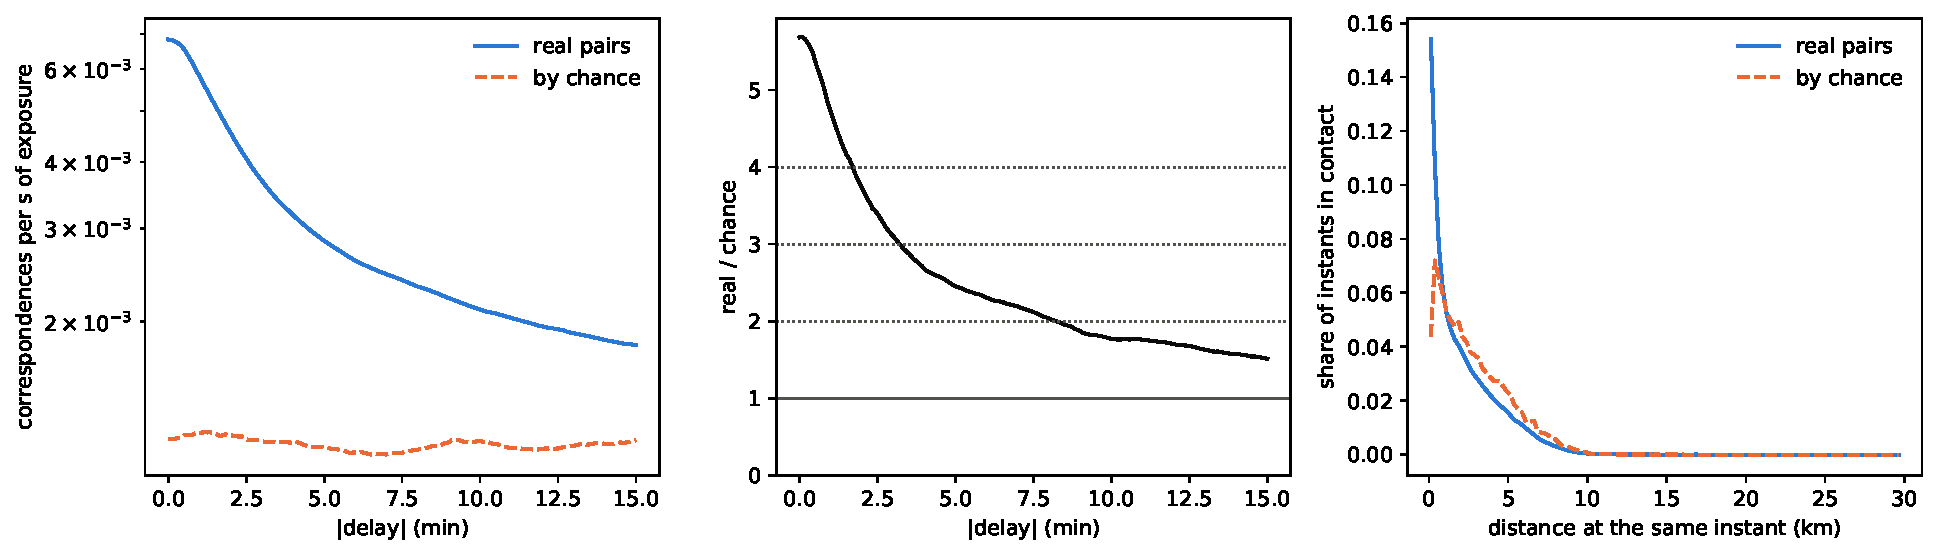
\includegraphics[width=0.98\textwidth]{tuning_delays.pdf}\\[2pt]
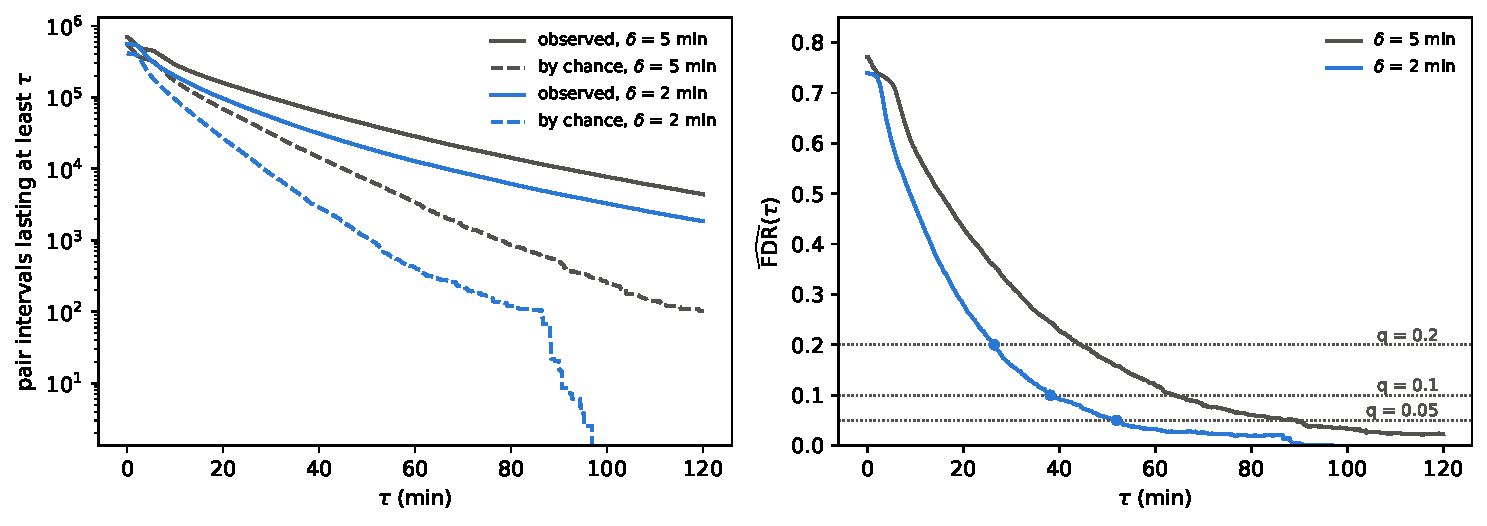
\includegraphics[width=0.78\textwidth]{tuning_fdr.pdf}
\caption{How the thresholds were set (tuning note). Top: correspondences per second at each delay,
real pairs against chance (left), their ratio (middle), distance at the same instant (right).
Bottom: real pair intervals lasting at least $\tau$ and those given by chance (left); estimated false
discovery rate (right), with $\tau^*$ for $q=0.05,0.1,0.2$.}
\label{fig:tuning}
\end{figure}

\textbf{Null model.} Pairs of flights of one day with takeoffs within 10~km (at most 200 per day)
are taken, and one flight of each pair is replaced by its own track shifted in time (at least
$2\delta+5$~s, so it cannot reproduce the real contact). Route, thermals and style are kept, the
interaction is not. The contacts of the copies are chance: scaled to the flying time of the real
pairs, day by day, they give $\widehat{\mathrm{FDR}}(\tau)$; $\tau^*$ is where it falls to $q$.
A contact is \emph{shared air within sight}, not proof of interaction: pilots who use the same
thermals at the same time without following each other survive the null model.

\subsection{Populations, strata and statistics}

\begin{itemize}
  \item \textbf{S} solo flights; \textbf{G} group time (stretches in a configuration);
        \textbf{A} the \emph{same flights alone} (stretches of group flights outside any
        configuration), the control with the same pilots, gliders, loggers and days; $\G_n$ the
        group time in configurations of $n$ pilots.
  \item \textbf{TA-MSD.} Positions on a 10~s grid of the flight clock; per flight
        $\overline{\delta^2}(\tau)=\sum\|\mathbf r(t+\tau)-\mathbf r(t)\|^2/\#\text{origins}$ pooled over
        its stretches, ensemble MSD = mean over flights (equal weight); stretches of at least
        1250~s, 21 lags from 10 to 1000~s. $H$: half the slope of $\log\mathrm{MSD}$ against $\log\tau$ over all lags
        ($H=1$ straight line). $H_\mathrm{loc}(\tau)$: the same slope on the lags within
        $\pm0.25$ decades of $\tau$ (Appendix~\ref{app:hloc}).
  \item \textbf{Phase statistics.} Ratios of sums over runs (time in climb, searches that end in a
        climb, climb rate, glide speed, glide ratio; cross-country speed over 30~min). Five of
        twelve are drawn: the others are explained by them (Appendix~\ref{app:redundancy}).
  \item \textbf{Strata.} \emph{Zone}: cell of 25~km of the middle of a piece of track;
        \emph{site-day}: flights of one day with takeoffs within 3~km; \emph{hour}: local hour.
  \item \textbf{Error bars} are 5--95\% bootstrap bands resampling whole \emph{blocks} (never
        flights) and recomputing the statistic: blocks of the note for pooled statistics (1000 draws);
        blocks joining episodes and site-days for stratified ones (200 draws, same draws for all).
        They measure block sampling only, not the choice of $q$ or the tolerances, and two bands that
        do not overlap are not a test; differences are computed draw by draw.
\end{itemize}

\textbf{What the grouping gives.} Of the 154\,598 paraglider flights with a logger of at most 10~s, 33\,501 (21.7\%) fly in a group at some point; of the 6\,039 hang-glider flights, 418 (6.9\%). Group time is 12.8\% of all paraglider flight time after the departure, and on average 45\% of the time of a group flight. The 36\,575 pair intervals last 40 to 96~min (10th to 90th percentile; median 52~min) and form 40\,051 configurations in 17\,169 episodes. Half of the episodes have two flights, 1\% have more than 9, the largest has 53. By the size of the configuration, the paraglider group time is: 2 pilots 64\%, 3 pilots 19\%, 4 pilots 8\%, 5-6 pilots 6\%, 7+ pilots 3\% (the largest configuration has 27 pilots). In contact, one pilot is behind the other by a median of 20~s (75\% within 45~s).


%======================================================================================
\section{Group or zone? Where the difference comes from}\label{sec:zones}

\textbf{Question.} Group time is more ballistic than solo flights at long lags. Is this the group, or the ground where groups fly
(and where solo pilots would also progress in a straight line)? \textbf{Method.} Each piece of track is assigned to a \emph{stratum} (zone = cell
of 25~km of its middle; zone$\times$month; zone$\times$hour; site-day$\times$hour). In every stratum with both populations the ensemble MSD
of the solo flights S (and of the same flights alone A) is \emph{reweighted to the mix of the group G over the strata}: S then flies, in
the statistic, where and when G flies. We compare $H_\mathrm{loc}(\tau)$ over \textbf{every lag} and the fitted $H$. The share of G with a counterpart
in its stratum is reported; ``as is'' is the same comparison without the reweighting, on the same strata and units (a flight counts once per
cell it crosses).

\begin{figure}[H]
\centering
\includegraphics[width=\textwidth]{zones_curves.pdf}
\caption{$H_\mathrm{loc}(\tau)$ of G (orange), of S reweighted to the strata of G (blue) and of A reweighted to them (green), 5--95\% bands.
First panel: all flights pooled (the raw comparison). ``Share of G kept'': flights of G with a solo counterpart in their stratum.}
\label{fig:zones}
\end{figure}

\begin{figure}[H]
\centering
\includegraphics[width=0.92\textwidth]{zones_differences.pdf}
\caption{$\Delta H_\mathrm{loc}(\tau)$ over every lag: G minus S (left) and G minus A (right), the other population reweighted to the strata of G; one line per
stratification, finer strata in darker orange.}
\label{fig:zones-diff}
\end{figure}

\begin{table}[H]
\centering\footnotesize\setlength{\tabcolsep}{2.6pt}
\begin{tabular}{@{}l r c c c c c c c c c@{}}
\toprule
 & & \multicolumn{3}{c}{fitted $H$ (10--1000 s)} & \multicolumn{3}{c}{$\Delta H$} & \multicolumn{3}{c}{$\Delta H_\mathrm{loc}(1000~\mathrm{s})$} \\
\cmidrule(lr){3-5}\cmidrule(lr){6-8}\cmidrule(l){9-11}
compared within & \makecell{G\\kept (\%)} & $\G$ & $\Sl\mid\G$ & $\A\mid\G$ & \makecell{$\G-\Sl$\\as is} & \makecell{$\G-\Sl$\\reweighted} & \makecell{$\G-\A$\\reweighted} & \makecell{$\G-\Sl$\\as is} & \makecell{$\G-\Sl$\\reweighted} & \makecell{$\G-\A$\\reweighted} \\
\midrule
none & 100 & 0.916 & 0.899 & 0.914 & $+$0.017 & \makecell{$+$0.017\\{\scriptsize[$+$0.016, $+$0.018]}} & \makecell{$+$0.002\\{\scriptsize[$+$0.001, $+$0.003]}} & $+$0.055 & \makecell{$+$0.055\\{\scriptsize[$+$0.053, $+$0.057]}} & \makecell{$+$0.032\\{\scriptsize[$+$0.030, $+$0.034]}} \\[2pt]
zone & 100 & 0.919 & 0.902 & 0.916 & $+$0.021 & \makecell{$+$0.018\\{\scriptsize[$+$0.017, $+$0.019]}} & \makecell{$+$0.003\\{\scriptsize[$+$0.003, $+$0.004]}} & $+$0.059 & \makecell{$+$0.056\\{\scriptsize[$+$0.054, $+$0.058]}} & \makecell{$+$0.028\\{\scriptsize[$+$0.026, $+$0.029]}} \\[2pt]
zone $\times$ month & 99 & 0.919 & 0.902 & 0.915 & $+$0.022 & \makecell{$+$0.017\\{\scriptsize[$+$0.016, $+$0.018]}} & \makecell{$+$0.003\\{\scriptsize[$+$0.003, $+$0.004]}} & $+$0.064 & \makecell{$+$0.054\\{\scriptsize[$+$0.053, $+$0.057]}} & \makecell{$+$0.028\\{\scriptsize[$+$0.027, $+$0.031]}} \\[2pt]
zone $\times$ hour & 99 & 0.919 & 0.902 & 0.913 & $+$0.022 & \makecell{$+$0.017\\{\scriptsize[$+$0.016, $+$0.018]}} & \makecell{$+$0.005\\{\scriptsize[$+$0.005, $+$0.006]}} & $+$0.064 & \makecell{$+$0.052\\{\scriptsize[$+$0.050, $+$0.054]}} & \makecell{$+$0.026\\{\scriptsize[$+$0.025, $+$0.028]}} \\[2pt]
site-day $\times$ hour & 53 & 0.917 & 0.904 & 0.913 & $+$0.015 & \makecell{$+$0.013\\{\scriptsize[$+$0.012, $+$0.014]}} & \makecell{$+$0.008\\{\scriptsize[$+$0.007, $+$0.009]}} & $+$0.051 & \makecell{$+$0.044\\{\scriptsize[$+$0.041, $+$0.046]}} & \makecell{$+$0.033\\{\scriptsize[$+$0.031, $+$0.036]}} \\[2pt]
\bottomrule
\end{tabular}

\caption{Fitted $H$ and differences by stratification. ``Reweighted'': the other population reweighted to the strata of G (value, 5--95\% band);
``as is'': the same strata without reweighting. $H_{\Sl\mid\G}$: $H$ of S reweighted to G.}
\label{tab:zones}
\end{table}

\begin{reading}
\textbf{Reading.}
\begin{itemize}
  \item \textbf{The gap opens above $\tau\approx150$~s.} $\Delta H_\mathrm{loc}(\tau)$ between G and S is small below it ($\ZoneShortMin$ to $\ZoneShortMax$ from 20 to 140~s)
        and rises to \ZoneDHlocSNone{} at 1000~s, above one climb--glide cycle: the group acts on how cycles are chained, not on a single glide or climb.
  \item \textbf{The zone does not explain it.} Reweighting S to the cells where G flies lowers $\Delta H_\mathrm{loc}(1000)$ by only \ZoneRedLocZone\%
        (\ZoneDHlocSupportZone{} $\to$ \ZoneDHlocSZone) and the fitted $\Delta H$ by \ZoneRedHZone\%; with the month, \ZoneRedLocZoneMonth\% and \ZoneRedHZoneMonth\%; with the
        hour, \ZoneRedLocZoneHour\% and \ZoneRedHZoneHour\%. At least 80\% of the long-lag gap remains. Solo pilots fly where groups fly: \ZoneKeptZone\% of G has a solo
        counterpart in its cell.
  \item \textbf{Same day, site and hour} (the finest strata, \ZoneKeptSdh\% of G kept): $\Delta H_\mathrm{loc}(1000)=\ZoneDHlocSSdh$ \ZoneDHlocSSdhBand, \ZoneRedLocSdh\% below its as-is value;
        fitted $\Delta H=\ZoneDHSSdh$ \ZoneDHSSdhBand. Solo flights on the same day, site and hour as a group still progress less straight over 1000~s.
  \item \textbf{Fitted $H$:} G \ZoneHNoneG{}, S \ZoneHNoneS{} raw. S reweighted to the zones of G: \ZoneHZoneS{}; to zone$\times$hour: \ZoneHZoneHourS{}; to site-day$\times$hour: \ZoneHSdhS{} (G \ZoneHSdhG).
        Reweighting raises the fitted $H$ of S by a few thousandths and never brings it to that of G.
  \item \textbf{Against the same flights alone} (A): $\Delta H_\mathrm{loc}(1000)$ is \ZoneDHlocANone{} pooled and \ZoneDHlocAZone, \ZoneDHlocAZoneHour, \ZoneDHlocASdh{} in zone, zone$\times$hour,
        site-day$\times$hour strata: the same pilots in the same zones and hours progress straighter in a group. Below 150~s the sign depends on the hour: A is above G pooled and equal at the same site-day and hour,
        which is why the within-flight estimate of Section~\ref{sec:other} must be read with the same-site-day-hour one.
  \item \textbf{Answer:} the difference between group and solo flights does not come from the zones where groups fly, nor from the month or hour at that place;
        it is reduced by about a fifth by the day, site and hour together, and the rest stays with the pilot and the day fixed. It is not a zone effect.
\end{itemize}
\textbf{Limits.} Cells are 25~km, from the middle of a piece; the terrain inside a cell (ridge, plain) is not controlled, and a group may choose better air within it:
this is part of what we call the group effect. Paragliders only.
\end{reading}


%======================================================================================
\section{Other statistics: what the group changes}\label{sec:other}

\begin{table}[H]
\centering\footnotesize
\begin{tabular}{@{}l l l l@{}}
\toprule
 & solo flights $\Sl$ & group time $\G$ & same flights alone $\A$ \\
\midrule
flights (TA-MSD) & 119\,129 & 33\,435 & 29\,611 \\
$H$ (10--1000~s) & 0.899 [0.898, 0.899] & 0.916 [0.915, 0.917] & 0.914 [0.913, 0.915] \\
$H_\mathrm{loc}(100~\mathrm{s})$ & 0.919 [0.919, 0.919] & 0.927 [0.927, 0.928] & 0.932 [0.931, 0.932] \\
$H_\mathrm{loc}(1000~\mathrm{s})$ & 0.837 [0.837, 0.838] & 0.893 [0.891, 0.894] & 0.860 [0.859, 0.862] \\
time in climb (\%) & 30.8 [30.7, 30.9] & 33.0 [32.8, 33.2] & 29.1 [28.9, 29.2] \\
searches ending in a climb (\%) & 43.3 [43.2, 43.4] & 49.5 [49.2, 49.7] & 45.9 [45.7, 46.1] \\
climb rate (m/s) & 1.22 [1.22, 1.22] & 1.26 [1.25, 1.27] & 1.33 [1.32, 1.34] \\
glide speed (km/h) & 30.1 [30.1, 30.2] & 33.3 [33.1, 33.5] & 32.8 [32.6, 32.9] \\
glide ratio & 10.4 [10.4, 10.4] & 12.9 [12.8, 13.0] & 11.3 [11.2, 11.4] \\
cross-country speed (km/h) & 17.2 [17.2, 17.3] & 20.0 [19.8, 20.3] & 20.0 [19.8, 20.1] \\
\bottomrule
\end{tabular}

\caption{Pooled statistics of S, G and A (paragliders), with 5--95\% bands (blocks of the note). TA-MSD on loggers of at most 10~s, phases on 1~Hz flights.}
\label{tab:raw}
\end{table}

\textbf{Design.} Five contrasts, each computed inside strata and averaged over those with both populations
(weights $n_Pn_Q/(n_P+n_Q)$, $n$ the flights of each side): $\G-\Sl$ pooled; $\G-\Sl$ and
$\A-\Sl$ (\emph{selection}) at the same site-day and hour; $\G-\A$ within the flight and at the same
site-day and hour (the \emph{group effect}, estimated in two ways that fail in opposite ways: the
first compares a flight with itself at another time of day, the second compares pilots at the same
time). Where the last two agree, the effect belongs to the group.

\begin{figure}[H]
\centering
\includegraphics[width=\textwidth]{decompose.pdf}
\caption{Each statistic (panel) for the five contrasts (rows), with 5--95\% bands. Shares of time in
points; lower height lost per km is a better glide.}
\label{fig:decompose}
\end{figure}

\begin{table}[H]
\centering\footnotesize\setlength{\tabcolsep}{3.5pt}
\begin{tabular}{@{}l c c c c c@{}}
\toprule
$\Delta$ & \makecell{$\G-\Sl$\\pooled} & \makecell{$\G-\Sl$\\same s-d-h} & \makecell{$\A-\Sl$\\same s-d-h} & \makecell{$\G-\A$\\same flight} & \makecell{$\G-\A$\\same s-d-h} \\
\midrule
$H_\mathrm{loc}(100~\mathrm{s})$ & \makecell{$+$0.008\\{\scriptsize[$+$0.007, $+$0.009]}} & \makecell{$+$0.002\\{\scriptsize[$+$0.001, $+$0.003]}} & \makecell{$+$0.005\\{\scriptsize[$+$0.004, $+$0.005]}} & \makecell{$-$0.009\\{\scriptsize[$-$0.009, $-$0.008]}} & \makecell{$+$0.002\\{\scriptsize[$+$0.001, $+$0.002]}} \\[2pt]
$H_\mathrm{loc}(1000~\mathrm{s})$ & \makecell{$+$0.055\\{\scriptsize[$+$0.053, $+$0.057]}} & \makecell{$+$0.041\\{\scriptsize[$+$0.038, $+$0.044]}} & \makecell{$+$0.003\\{\scriptsize[$+$0.001, $+$0.006]}} & \makecell{$+$0.037\\{\scriptsize[$+$0.035, $+$0.039]}} & \makecell{$+$0.043\\{\scriptsize[$+$0.040, $+$0.046]}} \\[2pt]
time in climb (\%) & \makecell{$+$2.20\\{\scriptsize[$+$1.96, $+$2.45]}} & \makecell{$+$3.43\\{\scriptsize[$+$3.19, $+$3.63]}} & \makecell{$+$0.43\\{\scriptsize[$+$0.25, $+$0.59]}} & \makecell{$+$5.71\\{\scriptsize[$+$5.52, $+$5.92]}} & \makecell{$+$3.28\\{\scriptsize[$+$3.11, $+$3.47]}} \\[2pt]
searches to climb (\%) & \makecell{$+$6.18\\{\scriptsize[$+$5.82, $+$6.46]}} & \makecell{$+$4.12\\{\scriptsize[$+$3.68, $+$4.54]}} & \makecell{$+$1.60\\{\scriptsize[$+$1.23, $+$1.97]}} & \makecell{$+$8.75\\{\scriptsize[$+$8.37, $+$9.15]}} & \makecell{$+$2.59\\{\scriptsize[$+$2.25, $+$2.99]}} \\[2pt]
climb rate (m/s) & \makecell{$+$0.040\\{\scriptsize[$+$0.030, $+$0.051]}} & \makecell{$+$0.031\\{\scriptsize[$+$0.025, $+$0.039]}} & \makecell{$+$0.007\\{\scriptsize[$+$0.001, $+$0.012]}} & \makecell{$+$0.024\\{\scriptsize[$+$0.019, $+$0.031]}} & \makecell{$+$0.029\\{\scriptsize[$+$0.025, $+$0.034]}} \\[2pt]
glide speed (km/h) & \makecell{$+$3.18\\{\scriptsize[$+$2.97, $+$3.39]}} & \makecell{$+$1.97\\{\scriptsize[$+$1.82, $+$2.10]}} & \makecell{$+$1.15\\{\scriptsize[$+$1.05, $+$1.27]}} & \makecell{$+$1.36\\{\scriptsize[$+$1.27, $+$1.46]}} & \makecell{$+$0.87\\{\scriptsize[$+$0.79, $+$0.98]}} \\[2pt]
height lost per km (m/km) & \makecell{$-$18.6\\{\scriptsize[$-$19.3, $-$17.8]}} & \makecell{$-$10.0\\{\scriptsize[$-$10.7, $-$9.1]}} & \makecell{$-$0.5\\{\scriptsize[$-$1.1, $+$0.3]}} & \makecell{$-$21.1\\{\scriptsize[$-$22.1, $-$20.1]}} & \makecell{$-$9.5\\{\scriptsize[$-$10.5, $-$8.6]}} \\[2pt]
cross-country speed (km/h) & \makecell{$+$2.81\\{\scriptsize[$+$2.59, $+$3.01]}} & \makecell{$+$2.25\\{\scriptsize[$+$2.09, $+$2.39]}} & \makecell{$+$1.31\\{\scriptsize[$+$1.21, $+$1.43]}} & \makecell{$+$0.70\\{\scriptsize[$+$0.60, $+$0.78]}} & \makecell{$+$1.29\\{\scriptsize[$+$1.16, $+$1.41]}} \\[2pt]
\bottomrule
\end{tabular}

\caption{The contrasts of Figure~\ref{fig:decompose}: difference and 5--95\% band (s-d-h: same site-day and hour).}
\label{tab:decompose}
\end{table}

\begin{reading}
\textbf{Reading.}
\begin{itemize}
  \item \textbf{Straighter progress over 1000~s} survives every control: $\Delta H_\mathrm{loc}(1000)$ is
        \DHlocThousandRaw{} pooled, \DHlocThousandFlight{} within the flight, \DHlocThousandGroupSdh{} at the same
        site-day and hour; selection only \DHlocThousandSel.
  \item \textbf{Nothing within one phase (100~s):} \DHlocHundredFlight{} within the flight,
        \DHlocHundredGroupSdh{} at the same place and hour; the pooled \DHlocHundredRaw{} was selection and composition.
  \item \textbf{More time climbing} (\DClimbFlight{}, \DClimbGroupSdh{} points) and \textbf{more searches that
        end in a climb} (\DFoundFlight{}, \DFoundGroupSdh{} points).
  \item \textbf{Climb rate is higher in a group} (\DRateFlight, \DRateGroupSdh{} m/s), not lower as in
        the pooled table: a composition effect (pooled ratios weight flights by their time in each population).
  \item \textbf{Faster and flatter glides:} \DSpeedFlight, \DSpeedGroupSdh{} km/h and \DSinkFlight, \DSinkGroupSdh{} m/km
        less height lost per km; selection adds \DSpeedSel{} km/h of glide speed (group pilots glide faster even alone).
  \item \textbf{Cross-country speed} is higher in a group once stratified: \DXcFlight, \DXcGroupSdh{} km/h.
\end{itemize}
\end{reading}

%--------------------------------------------------------------------------------------
\subsection{Size of the configuration}\label{sec:size}

The group time is cut where the configuration changes: every stretch has a fixed number of pilots $n$
(2, 3, 4, 5--6, 7+); a flight can contribute to several sizes. Two contrasts by size: each size minus the
same flights alone (within the flight), and each size minus configurations of 2 pilots (same site-day
and hour: does the size matter beyond a pair?).

\begin{figure}[H]
\centering
\includegraphics[width=0.56\textwidth]{size_hloc.pdf}
\caption{$H_\mathrm{loc}(\tau)$ over every lag by the size of the configuration (orange, darker with more pilots), S (blue) and, dashed, the same
flights alone for each size.}
\label{fig:size-hloc}
\end{figure}

\begin{table}[H]
\centering\footnotesize\setlength{\tabcolsep}{3pt}
\begin{tabular}{@{}l r c c c c c c c c c@{}}
\toprule
 & & \multicolumn{2}{c}{$H$} & \multicolumn{2}{c}{$H_\mathrm{loc}(1000~\mathrm{s})$} & & & & & \\
\cmidrule(lr){3-4}\cmidrule(lr){5-6}
pilots & flights & $\G_n$ & alone & $\G_n$ & alone & \makecell{time in\\climb (\%)} & \makecell{searches\\to climb (\%)} & \makecell{climb\\rate (m/s)} & \makecell{glide speed\\(km/h)} & \makecell{glide\\ratio} \\
\midrule
solo & 119\,129 & 0.899 &  & 0.837 &  & 30.8 & 43.3 & 1.22 & 30.1 & 10.4 \\
2 & 26\,411 & 0.917 & 0.914 & 0.889 & 0.861 & 32.7 & 49.0 & 1.27 & 33.2 & 12.5 \\
3 & 9\,480 & 0.923 & 0.919 & 0.906 & 0.867 & 33.6 & 49.9 & 1.26 & 33.5 & 13.1 \\
4 & 4\,073 & 0.924 & 0.920 & 0.910 & 0.865 & 33.6 & 51.0 & 1.25 & 33.5 & 13.7 \\
5--6 & 2\,686 & 0.925 & 0.922 & 0.915 & 0.870 & 33.1 & 50.1 & 1.23 & 33.1 & 14.1 \\
7+ & 1\,142 & 0.933 & 0.924 & 0.944 & 0.871 & 34.6 & 51.7 & 1.20 & 34.6 & 15.9 \\
\bottomrule
\end{tabular}

\caption{Paragliders, pooled by the size of the configuration (``alone'': the same flights alone).}
\label{tab:size}
\end{table}

\begin{figure}[H]
\centering
\includegraphics[width=\textwidth]{decompose_size.pdf}
\caption{Orange: $\G_n-\A$ within the flight. Blue: $\G_n-\G_2$ at the same site-day and hour.}
\label{fig:size}
\end{figure}

\begin{reading}
\textbf{Reading.} Pooled, $H$ and $H_\mathrm{loc}$ rise with $n$ while the same flights alone stay flat (Fig.~\ref{fig:size-hloc}, Table~\ref{tab:size}). Within the flight the straight-progress effect grows with $n$ (\DHlocThousandFlightTwo{} with 2 pilots,
\DHlocThousandFlightSeven{} with 7+), but at the same site-day and hour configurations of 3 to 6 pilots do not differ from pairs
($\Delta H_\mathrm{loc}(1000)$ between \DHlocThousandMiddleMin{} and \DHlocThousandMiddleMax, bands across zero): the rise
of the pooled curves belongs to the days and sites where large groups form. Only 7+ stands apart
(\DHlocThousandSevenTwoSdh{} \DHlocThousandSevenTwoSdhBand, cross-country speed \DXcSevenTwoSdh{} km/h), a rare
configuration (3\% of group time) of unknown nature. Time in climb and the flatter glide do grow with $n$ at the same place
and hour (\DClimbSizeMin{} to \DClimbSizeMax{} points; \DSinkSizeMin{} to \DSinkSizeMax{} m/km).
\end{reading}

%--------------------------------------------------------------------------------------
\subsection{How groups form and break, who leads, when they fly}\label{sec:mechanisms}

\begin{itemize}
  \item \textbf{Entering and leaving.} The phase at the instant a flight enters (\Entries{}) or leaves (\Exits{}) a group,
        against the time shares; entries and exits at the departure or the landing apart (\AtDeparture{}, \AtLanding{}).
  \item \textbf{Leader and follower.} In configurations of two pilots the signed median delay of the pair
        interval says who passes first (leader: the other passes at least 15~s later; \Abreast\% abreast, median
        delay \DelayMedian~s). The two are compared within the configuration.
  \item \textbf{Habitual leaders.} For the \HabitualPilots{} pilots with at least 10 roles in pairs: dispersion of the
        lead fractions against roles swapped at random.
  \item \textbf{Hours.} Time of S, A and G over the local hour.
\end{itemize}

\begin{figure}[H]
\centering
\includegraphics[width=0.49\textwidth]{mechanisms_phases.pdf}\hfill
\includegraphics[width=0.49\textwidth]{mechanisms_habitual.pdf}\\[3pt]
\includegraphics[width=0.9\textwidth]{mechanisms_hours.pdf}
\caption{Top left: phase at entry and exit against the time shares (bands: blocks). Top right: lead fraction of each
pilot, against roles at random. Bottom: time over the local hour (left) and share spent in a group (right).}
\label{fig:mechanisms}
\end{figure}

\begin{reading}
\textbf{Reading.}
Entries fall in climbs \PhaseEntryClimb\%, searches \PhaseEntrySearch\% and glides \PhaseEntryTransition\% of the cases, exits
\PhaseExitClimb, \PhaseExitSearch, \PhaseExitTransition\%, against \PhaseAloneClimb, \PhaseAloneSearch, \PhaseAloneTransition\% of the time alone:
\textbf{no phase where groups preferentially form or break}. \EntriesEarly\% of entries are within 10~min of the departure.
The pilot ahead flies a little faster (glide speed \LeadSpeed{} km/h, climb rate \LeadRate{} m/s) but does not find thermals more
often (searches ending in a climb \LeadFound{} points, height lost per km \LeadSink{} m/km): within a pair the follower
shows no sign of using the leader to find the next thermal. Dispersion of lead fractions \HabitualDispersion{} against
\HabitualNull{} at random (95\% below \HabitualNullHigh): \textbf{some pilots lead or follow persistently} (\HabitualExtreme\% lead in at
most 20\% or at least 80\% of their roles, \HabitualExtremeNull\% expected). Group time is concentrated around midday
(\GroupShareNoon\% of a group flight's time at \GroupShareNoonHour~h, \GroupShareMorning\% at 9~h, \GroupShareEvening\% at 18~h), and its time alone
falls earlier and later: this is why $\G-\A$ within the flight must be read with the same-site-day-hour estimate.
\end{reading}


%======================================================================================
\section{Conclusions and limits}\label{sec:conclusions}

\begin{minipage}[t]{0.49\textwidth}
\textbf{Supported}
\begin{itemize}
  \item the progress over a quarter of an hour is straighter in a group, with the pilot, the day,
        the site and the hour fixed;
  \item no effect within one glide or climb (100~s) at the same hour;
  \item more time climbing, more searches that end in a climb, faster and flatter glides;
  \item climb rate and cross-country speed are \emph{higher} in a group once the composition is
        controlled (the pooled readings reversed);
  \item selection of pilots is small for the motion;
  \item groups form and break in every phase; some pilots lead persistently.
\end{itemize}
\end{minipage}\hfill
\begin{minipage}[t]{0.49\textwidth}
\textbf{Not supported}
\begin{itemize}
  \item that the group \emph{causes} the effect: the strata fix pilot, day, site, hour and zone, not
        the decision to fly together;
  \item that larger groups straighten the progress, up to six pilots;
  \item that a contact means interaction (shared air within sight);
  \item the glide statistics are partly by definition (aligned headings in glide);
  \item phases exist on 1~Hz flights only; the same analyses on the xc-dynamics tracks are open.
\end{itemize}
\end{minipage}

\clearpage
\appendix
%======================================================================================
\section{How $H$ and $H_\mathrm{loc}$ are computed}\label{app:hloc}

$\mathrm{MSD}(\tau)\propto\tau^{2H}$, so $\log_{10}\mathrm{MSD}=2H\log_{10}\tau+c$. \textbf{$H$} is half the slope of the
least-squares line over all 21 lags (equal weight per lag). \textbf{$H_\mathrm{loc}(\tau_c)$} is half the slope of the line fitted on
the lags with $|\log_{10}\tau-\log_{10}\tau_c|\le0.25$ (a factor 1.78 on each side), equal weight; where fewer than
3 lags lie in the window, the 3 nearest are used. It is a windowed regression, not a pointwise derivative.
$\Delta H$ and $\Delta H_\mathrm{loc}$ of two curves are the differences of the fitted values; for a stratified
average they are the same regression on the averaged $\Delta\log\mathrm{MSD}$ (linear: slope of a difference = difference of slopes).
Bands: the same computation on each bootstrap draw, percentiles lag by lag.

\begin{table}[H]
\centering\footnotesize
\begin{tabular}{@{}r l@{\hspace{14pt}}r l@{\hspace{14pt}}r l@{}}
\toprule
$\tau$ (s) & lags used & $\tau$ (s) & lags used & $\tau$ (s) & lags used \\
\midrule
10 & 10--30 (3 nearest) & 90 & 60--140 & 320 & 210--470 \\
20 & 20--40 (3 nearest) & 100 & 60--170 & 390 & 260--580 \\
30 & 20--50 & 110 & 80--170 & 470 & 320--710 \\
40 & 30--60 & 140 & 80--210 & 580 & 390--1000 \\
50 & 30--80 & 170 & 100--260 & 710 & 470--1000 \\
60 & 40--100 & 210 & 140--320 & 870 & 580--1000 \\
80 & 50--140 & 260 & 170--390 & 1000 & 580--1000 \\
\bottomrule
\end{tabular}
\caption{Lags of the window of each $H_\mathrm{loc}$ value. At 10 and 20~s the window is not centred; at 870 and 1000~s
it is cut at 1000~s and the two values use the same lags, so the end of the curve flattens by construction. The window
resolves nothing narrower than about half a decade.}
\end{table}

\textbf{Phase MSD figures (not in this report)} use a different local exponent: the finite-difference derivative of $\log\mathrm{MSD}$
against $\log\Delta$ on 100 lags, without the factor $1/2$ (about 2 for ballistic motion).

\textbf{Ratios and the glide ratio.} Ratios are sums of numerators over sums of denominators over the runs of a population (a run
goes to the stretch that holds its middle). In a small stratum a glide in rising air has almost no height lost, the glide ratio
diverges and its average over strata is unstable; stratified contrasts use the \emph{height lost per km of glide}, the inverse. Pooled tables keep the glide ratio.

%======================================================================================
\section{Checks of the grouping and of the viewer}\label{app:audit}

\begin{itemize}
  \item \textbf{Code against the methodological note.} Every phase was compared with its code (grid, departure, candidate filter, scan of delays,
        contact, gaps, signed delay, null model, configurations, episodes, membership, blocks): all implemented as written, with four differences of text, \textbf{now
        corrected in red in the note}:
        (1) the phases of the run are Vilpellet's, on 1~Hz flights, not the hidden Markov model of xc-lab, so the heading condition acts only between two such flights;
        (2) headings are in the east and north of the first fix of each flight, not of the fix itself (a rotation of about $3^\circ$ at 300~km, against 45$^\circ$);
        (3) a contact is kept only from the later departure to the earlier landing (at most $\delta$ lost at the ends);
        (4) instants in a gap of the track are labelled solo in the tables.
  \item \textbf{Properties of the tables} (chosen run): every pair interval lasts at least $\tau^*=2285$~s and lies where both flights fly after departure; every configuration has at least
        two members; membership covers each flight from takeoff to landing without holes; on 3\,000 flights the group time equals the union of its pair intervals; on 3\,000 configurations the members are
        connected at the midpoint and no active interval leaves; on 2\,000 episodes every configuration but the first starts when another ends and shares a member; every episode lies in one block. The
        counts of the note (154\,598 and 6\,039 flights; 21.7\% and 6.9\% in a group) are reproduced.
  \item \textbf{Viewer.} The \emph{Group flights} tab reads \texttt{groups/} of its data folder: its seven tables are \textbf{byte-identical} to those of the chosen run; the tracks it draws (\texttt{SSD\_DATA}) have the same fixes,
        times, positions and trimmed starts as those the grouping read (\texttt{SSD\_DISANTE}).
  \item \textbf{Analyses.} Tests on synthetic flights for every step, and on every number of the README of the analyses; the decomposition is checked on a synthetic case where the day raises
        a statistic by 10 and the group by 2: pooled 10, stratified 2.
\end{itemize}

%======================================================================================
\section{Which statistics are drawn}\label{app:redundancy}

Unit: a population on a site-day with at least 25 flights (119 units). A statistic is redundant when the others explain most of it across units ($R^2$ of its linear
regression on them); backward elimination drops the most explained until every $R^2\le0.5$. The four shares of time sum to 100\%, so one of them goes first.

\begin{table}[H]
\centering\footnotesize
\begin{tabular}{@{}l l c@{}}
\toprule
statistic & status & R$^2$ on the five drawn \\
\midrule
time in climb (\%) & drawn & 0.23 \\
searches that end in a climb (\%) & drawn & 0.41 \\
climb rate (m/s) & drawn & 0.20 \\
glide speed (km/h) & drawn & 0.26 \\
glide ratio & drawn & 0.38 \\
time in transition (\%) & dropped, number 1, R$^2$ 1.00 when dropped & 0.83 \\
height gained per climb (m) & dropped, number 2, R$^2$ 0.98 when dropped & 0.91 \\
climbs that start after a search (\%) & dropped, number 3, R$^2$ 0.93 when dropped & 0.77 \\
cross-country speed over 30 min (km/h) & dropped, number 4, R$^2$ 0.93 when dropped & 0.90 \\
time in a search in vain (\%) & dropped, number 5, R$^2$ 0.88 when dropped & 0.71 \\
climbs per hour & dropped, number 6, R$^2$ 0.72 when dropped & 0.71 \\
time in a search that ends in a climb (\%) & dropped, number 7, R$^2$ 0.65 when dropped & 0.65 \\
\bottomrule
\end{tabular}

\caption{Five statistics remain; the others are explained by them.}
\end{table}

%======================================================================================
\section{Pooled curves, hang gliders and sizes}\label{app:curves}

\begin{figure}[H]
\centering
\includegraphics[width=0.78\textwidth]{tamsd.pdf}
\caption{TA-MSD and $H_\mathrm{loc}$ of S, G and A, paragliders and hang gliders (hang gliders: 418 group flights, wide bands at long lags).}
\end{figure}

\begin{figure}[H]
\centering
\includegraphics[width=0.78\textwidth]{size_tamsd.pdf}
\caption{By the size of the configuration (orange, darker with more pilots), S (blue) and, dashed, the same flights alone for each size.}
\end{figure}


%======================================================================================
\section{Single site-days}\label{app:sitedays}

Six site-days chosen by a fixed rule (most sizes with 15 flights or more, then most flights, at most two per takeoff site). Bands resample flights (too narrow: flights of one group are not independent).

\begin{figure}[H]
\centering
\includegraphics[width=0.9\textwidth]{siteday_tamsd.pdf}
\caption{TA-MSD and $H_\mathrm{loc}$ on six site-days by the size of the configuration, with the solo flights of the same site-day where they reach 15 flights.}
\end{figure}

\begin{table}[H]
\centering\footnotesize
\begin{tabular}{@{}l l l l l l l@{}}
\toprule
site-day & solo & 2 & 3 & 4 & 5--6 & 7+ \\
\midrule
Saint Hilaire sud, 2022-03-26 & 0.750 & 0.853 & 0.894 & 0.818 &  & 0.994 \\
Saint Hilaire sud, 2017-03-28 & 0.854 & 0.931 & 0.901 & 0.956 &  & 0.873 \\
M\'eruz, 2019-05-01 &  & 0.926 & 0.939 &  & 0.938 &  \\
M\'eruz, 2016-04-28 &  & 0.894 & 0.958 &  & 0.957 &  \\
Chalvet Ouest, 2016-07-19 &  & 0.951 &  &  & 0.892 &  \\
La Sambuy, 2020-07-25 &  & 0.941 & 0.901 &  &  &  \\
\bottomrule
\end{tabular}

\caption{$H_\mathrm{loc}(1000~\mathrm{s})$ by size on each site-day (empty: fewer than 15 flights). Differences between days exceed those between sizes (the climb rate goes from 0.79 to 2.11~m/s across the six days).}
\end{table}

%======================================================================================
\section{Robustness to the threshold}\label{app:robustness}

With $q=0.2$ contacts need to last only 26.4~min: more and shorter groups, up to one contact in five chance.

\begin{table}[H]
\centering\footnotesize
\begin{tabular}{@{}l l l@{}}
\toprule
 & $q=0.1$, $\tau^*=38.1$~min & $q=0.2$, $\tau^*=26.4$~min \\
\midrule
group flights (TA-MSD) & 33\,435 & 48\,777 \\
$H_\mathrm{loc}(1000~\mathrm{s})$, $\Sl$ & 0.837 & 0.836 \\
$H_\mathrm{loc}(1000~\mathrm{s})$, $\A$ & 0.860 & 0.854 \\
$H_\mathrm{loc}(1000~\mathrm{s})$, $\G$ & 0.893 & 0.892 \\
$\Delta H_\mathrm{loc}(1000~\mathrm{s})$, $\G-\A$ same flight & $+$0.037 [$+$0.035, $+$0.039] & $+$0.032 [$+$0.029, $+$0.035] \\
$\Delta H_\mathrm{loc}(1000~\mathrm{s})$, $\G-\A$ same s-d-h & $+$0.043 [$+$0.040, $+$0.046] & $+$0.042 [$+$0.040, $+$0.044] \\
$\Delta H_\mathrm{loc}(1000~\mathrm{s})$, $\A-\Sl$ same s-d-h & $+$0.003 [$+$0.001, $+$0.006] & $+$0.002 [$-$0.001, $+$0.005] \\
$\Delta H_\mathrm{loc}(100~\mathrm{s})$, $\G-\A$ same flight & $-$0.009 [$-$0.009, $-$0.008] & $-$0.016 [$-$0.017, $-$0.015] \\
$\Delta H_\mathrm{loc}(100~\mathrm{s})$, $\G-\A$ same s-d-h & $+$0.002 [$+$0.001, $+$0.002] & $-$0.004 [$-$0.005, $-$0.003] \\
$\Delta$ searches to climb, $\G-\A$ same s-d-h (points) & $+$2.6 [$+$2.3, $+$3.0] & $+$3.4 [$+$3.0, $+$3.7] \\
$\Delta$ climb rate, $\G-\A$ same s-d-h (m/s) & $+$0.029 [$+$0.025, $+$0.034] & $+$0.024 [$+$0.020, $+$0.029] \\
$\Delta$ height lost per km, $\G-\A$ same s-d-h (m/km) & $-$9.5 [$-$10.5, $-$8.6] & $-$11.5 [$-$12.2, $-$10.9] \\
$\Delta$ cross-country speed, $\G-\A$ same s-d-h (km/h) & $+$1.29 [$+$1.16, $+$1.41] & $+$1.14 [$+$1.01, $+$1.30] \\
\bottomrule
\end{tabular}

\caption{The main results with the two thresholds (s-d-h: same site-day and hour). Every conclusion keeps its sign; at 100~s both estimates of the group effect are slightly negative with $q=0.2$: no robust effect within one phase.}
\end{table}

%======================================================================================
\section{Leader minus follower}\label{app:leaders}

\begin{figure}[H]
\centering
\includegraphics[width=0.95\textwidth]{mechanisms_leaders.pdf}
\caption{Leader minus follower, same configuration of two pilots.}
\end{figure}

\begin{table}[H]
\centering\footnotesize
\begin{tabular}{@{}l l@{}}
\toprule
$\Delta$ & leader $-$ follower \\
\midrule
$H_\mathrm{loc}(100~\mathrm{s})$ & $-$0.002 [$-$0.002, $-$0.001] \\
$H_\mathrm{loc}(1000~\mathrm{s})$ & $-$0.003 [$-$0.004, $-$0.001] \\
time in climb (\%) & $+$0.91 [$+$0.57, $+$1.25] \\
searches ending in a climb (\%) & $-$0.01 [$-$1.03, $+$0.83] \\
climb rate (m/s) & $+$0.021 [$+$0.014, $+$0.028] \\
glide speed (km/h) & $+$0.86 [$+$0.74, $+$0.99] \\
height lost per km of glide (m/km) & $+$1.6 [$-$0.9, $+$4.5] \\
cross-country speed (km/h) & $+$0.14 [$+$0.11, $+$0.16] \\
\bottomrule
\end{tabular}

\caption{Leader minus follower, same configuration of two pilots (difference with 5--95\% band).}
\end{table}

\begin{table}[H]
\centering\footnotesize
\begin{tabular}{@{}l l l l@{}}
\toprule
 & climb (\%) & search (\%) & transition (\%) \\
\midrule
entering a group & 28.1 [27.6, 28.5] & 10.3 [10.0, 10.6] & 61.5 [61.0, 61.9] \\
leaving a group & 28.0 [27.6, 28.3] & 11.2 [10.9, 11.5] & 60.6 [60.1, 61.0] \\
share of time, alone & 29.1 [28.9, 29.3] & 10.1 [10.0, 10.2] & 60.8 [60.6, 61.0] \\
share of time, in a group & 33.0 [32.8, 33.2] & 9.4 [9.2, 9.6] & 57.6 [57.3, 57.9] \\
\bottomrule
\end{tabular}

\caption{Phase at the instant of entering or leaving a group, and shares of time in each phase (percent, with 5--95\% bands).}
\end{table}

%======================================================================================
\section{Reproducing the report}\label{app:reproduce}

From \texttt{xc-lab/analyses/groups}, SSD\_DISANTE mounted:
\begin{verbatim}
uv run python tamsd.py; uv run python phase_msd.py; uv run python survival.py
uv run python budget.py; uv run python performance.py; uv run python blocks.py
uv run python redundancy.py; uv run python size.py; uv run python decompose.py
uv run python zones.py; uv run python mechanisms.py; uv run python report/facts.py
uv run python report/tables.py; cd report; latexmk -pdf group_vs_solo.tex
\end{verbatim}
Heavy pieces stay on SSD\_DISANTE, in the \texttt{analyses/} folder of each run; figures and JSON in \texttt{out/<run>/}.


\end{document}
